% !TEX root = ../thesis.tex

\chapter{Implementation} \label{implementation}

The primary language used to implement Intertext is Typescript. Typescript is a superset of Javascript that brings it typing support for safety and a better developer experience. Typescript gets transpiled into Javascript during build time, therefor the byproduct is plain Javascript. Sharing the same language between Intertext clients brings a number of advantages, mostly code sharing.

\section{Engine}

Code sharing between Intertext clients has been an important priority while creating the architecture for several reasons. First of all, it is crucial for Intertext clients to behave consistently for some tasks that are common to every Intertext client, such as parsing of IUIDL, rendering of the components, behavioural aspects of the clients, the data structure and so on. These are the cornerstone of Intertext, and they must behave exactly the same across clients. In another words, everything that isn't client-specific needs to be consistent and predictable. This is where Intertext engine comes in play.

Intertext engine implements several aspects of Intertext clients; most notably it parses IUIDL, internally converts it into JSON, and uses the output to render the components. Intertext clients are only concerned with the view layer, but they use the engine as a black box system. The engine also defines the data types of every component, and internal mechanics of the build and rendering process. It exposes the types for Intertext clients built with Typescript to consume. Intertext engine is built as a standalone library, it exposes the main functions and types, and it is designed to be used in several different ways.

At the time of writing, all Intertext clients that are implemented so far were built with Typescript, they simply import and use the engine as a dependency. Their build system picks up the engine and adds it to their final bundle. However this approach is not possible for potential future clients that do not built on a Javascript runtime. To overcome this issue, the engine can be compiled as a Node module, and be deployed to a Node.js server. This gives us the ability to use the engine on any software system that can send or receive HTTP requests. Moreover, with the same logic, the engine can be deployed locally alongside any Intertext client that runs on a platform that can support Node.js runtime. It can then be deployed and served locally, and used to communicate with the local Intertext client using any protocol that is supported by the host platform as long as there exists a data exchange. 

For instance, let's say a car manufacturer wanted to build an Intertext client for their in-car entertainment system using their own components. They could potentially install Node.js on their computer system, or even install a simple raspbery-pi like chip that can run Node.js. Then, they can install the engine as a standalone application in it, and utilize any protocol to build a communication channel between the Intertext client they built on their computer system and the chip. Then, they could serve the IUIDL code either through a network connection (if and when available), or from a locally running server, potentially from the same one the client uses to interact with the engine. 

\section{Layout}

The premise of Intertext is that there will be a unified implementation of UI, in a more or less abstract format, which will then be reified into fully functional front-ends on many different environments. These environments have different requirements and limitations; and an all-in-one solution is needed that will handle all these different requirements and limitations with minimal compromises. One of the aspects that needed consideration was the variation in screen sizes. We had to use a layout system that can be used to build a UI once, and would render properly on various screen sizes.

The obvious solution to this problem was using web technologies, as responsive design is one of the cornerstones of web development. There are many well defined specifications in place to build UI's for different screen sizes. But we cannot directly use web technologies as many of the clients are not browser based. Therefor, we had to use an hybrid approach that can work universally.

\subsection{Layout System}

IUIDL offers a powerful layout system based on the css flexbox specification. It allows developers to build responsive layouts and position UI elements with ease. Intertext web client makes use of the browser implementation of CSS flexbox, whereas for other non-browser based clients, we use Facebook's open source library Yoga \cite{FacebookYoga}. Yoga is a layout engine that implements css flexbox specifications in C++, therefor it can be used on any ecosystem that can execute C++ to calculate the positioning of the UI elements. We currently use Yoga layout engine indirectly on our command-line client, for it was built with a framework that internally uses the Yoga engine.

\begin{figure}[H]
  \centering
  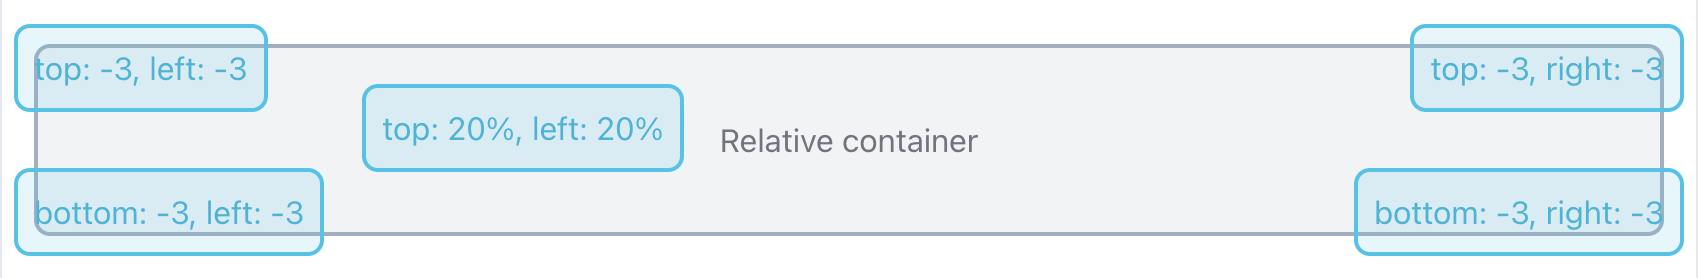
\includegraphics[width=13cm]{thesis/paper/images/absolute.png}
  \caption{Absolute positioning}%
  \label{fig:flexbox_props}%
\end{figure}

Apart from flexbox-based positioning, Intertext layout system also supports absolute positioning. Absolute positioning, as opposed to relative positioning, detaches a component from the flow of the page and positions it relative to its first relatively-positioned parent, having it be floating over everything else, as shown in Figure \ref{fig:absolute_positioning}.

\begin{figure}
  \centering
  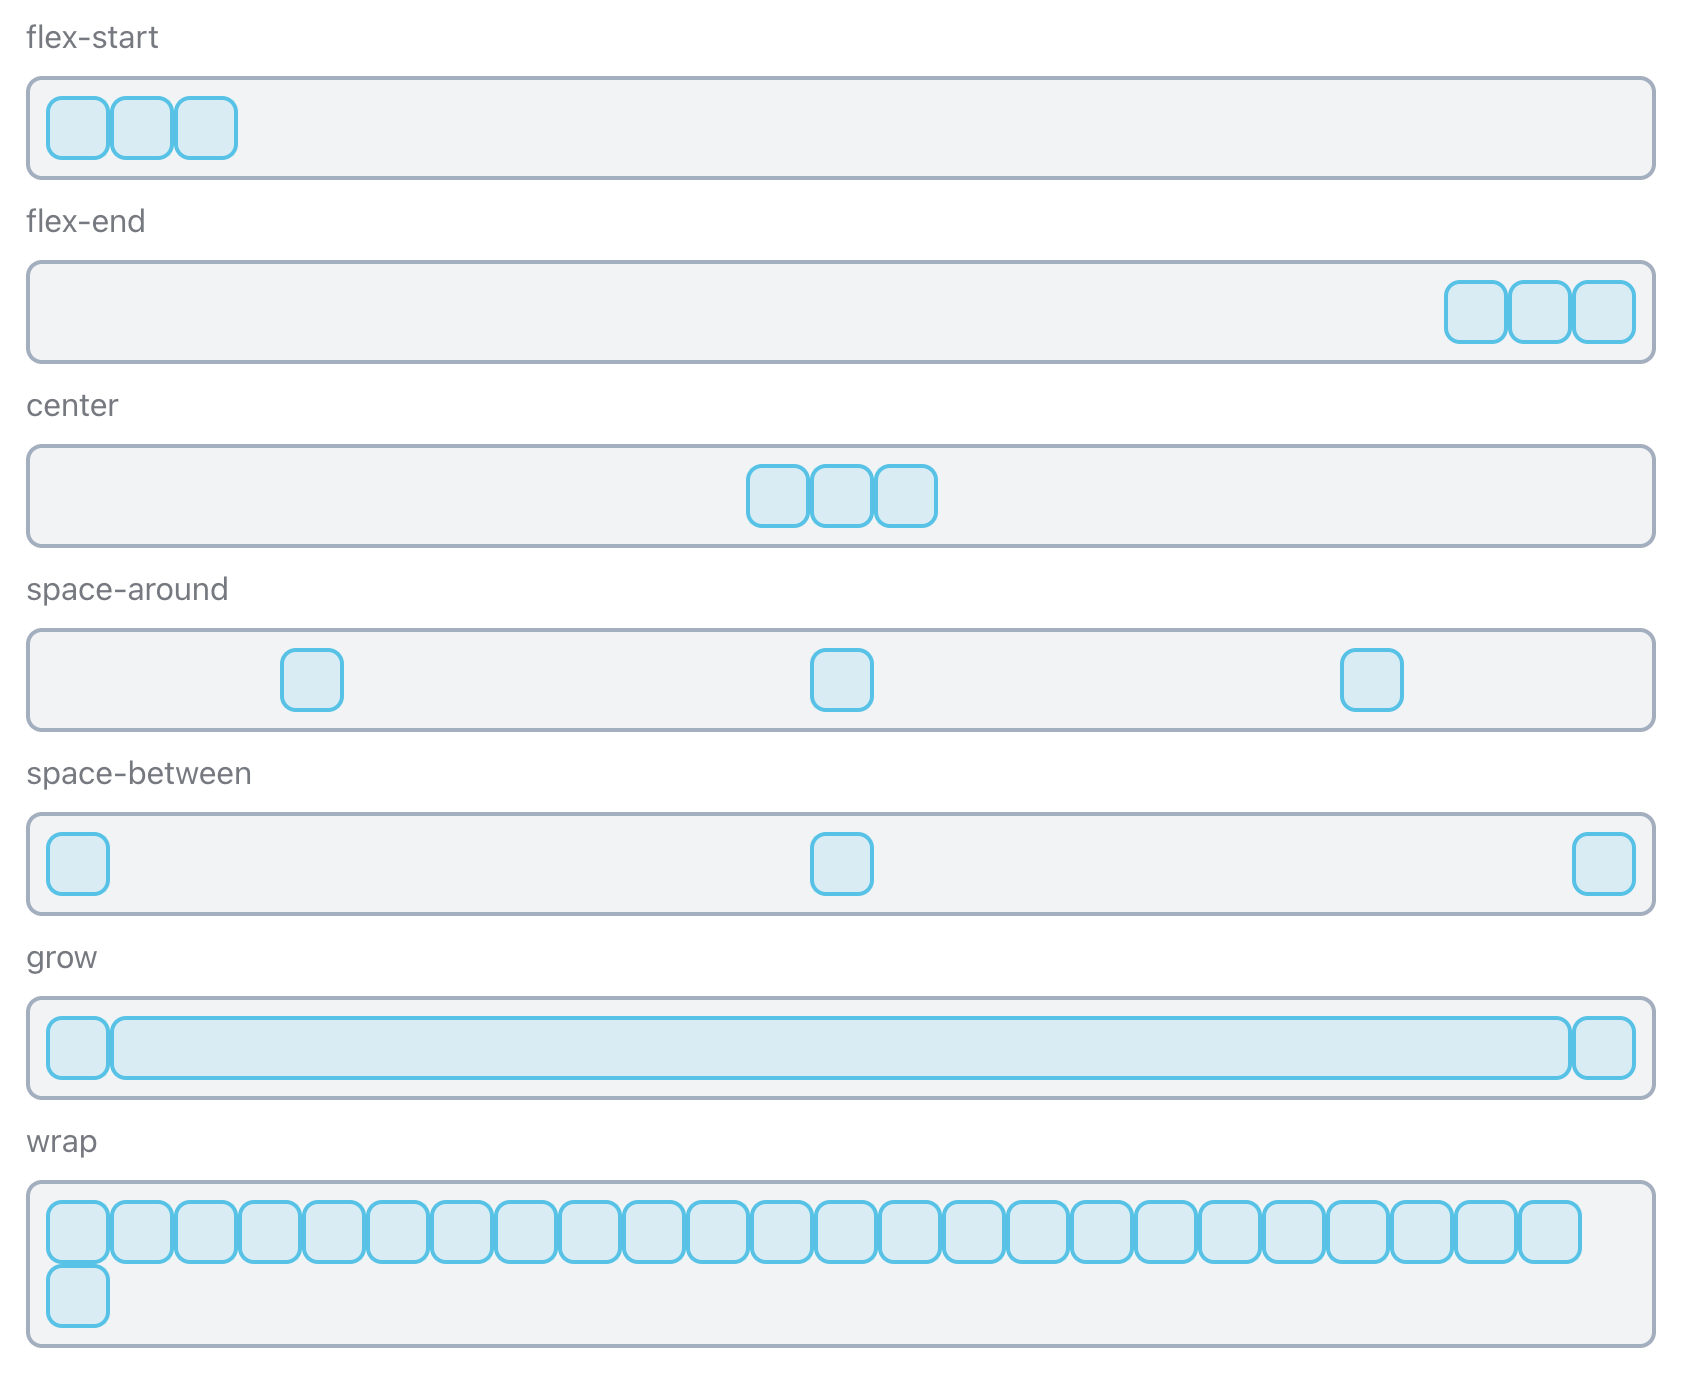
\includegraphics[width=13cm]{thesis/paper/images/responsive.png}
  \caption{Flexbox system}%
  \label{fig:absolute_positioning}%
\end{figure}

One advantage to this approach is that all our clients will render UI elements using the same layout, which will give users a sense of familiarity when switching between the clients. For instance, when a user accustomed to using the web version of Intertext switches to, say the command-line version, they will immediately recognise the layout and be able to navigate without having to adjust. This approach will also allow developers to build responsive layouts to some extent. Given that the same UIDL code will be used to render on multiple clients including ones with narrow and small screens, responsiveness goes a long way. At the time of writing, only flexbox features such as "flex-wrap" can be used for achieving a degree of responsiveness. However we plan to support screen-size aware variants of component properties, even conditional rendering of components based on the screen size. This can be thought of as "media queries" in css terminology. More on this will be on the \nameref{futureWork} section.

\subsection{Unit System}

One of the compromises we had to make for our an all-in-one layout solution was the unit system. We refrained from using definitive units that are specific to one platform, such as pixels. Most platforms use a different measurement system, for instance 1 unit for command-line applications represents a single space; character width for the x-axis and line height for the y-axis.

As a solution, we offer three different types of units; percentages, spaces and sizes. These units can be used for every property that accepts a unit; such as for width, height, margins, paddings and so on. Percentages are universal and can be calculated on any platform that we can get the screen dimensions of. We are able to use it in web environment natively, also the Yoga engine supports percentage values. Spaces are numeric values that starts from 0, increments by 0.5 until 4, by 1 until 12, by 2 until 16, and keeps increasing exponentially until 96. These values are meant to be used for spacing; for paddings, margins, gutter sizes, and other cases where spaces between UI elements needs to be determined. They are mapped to values on different platforms that are reasonable and look approximately same. Finally, we have sizes, which are used for determining the size of UI elements; in properties such as width, height, minWidth/maxWidth, minHeight/maxHeight and so on. While it also makes sense to use percentages for sizes, in cases where sizes should be fixed and not be changing based on the screen size, the size units can be used. Sizes are named values and are mapped to an appropriate value on every platform. They start from 3xs (xsmall) - up to xs, sm (small), md (medium), lg (large), xl (xlarge), 2xl and goes all the way to 8xl.

\subsection{Layout Properties}

\begin{figure}[H]
\begin{minipage}{\linewidth}
\begin{lstlisting}[language=xml]
<block height="24" alignItems="center" justifyContent="center">
  <text>This is centered</text>
</block>
\end{lstlisting}
\end{minipage}
\caption{Layout properties}%
\label{fig:layout_props_example}%
\end{figure}

IUIDL defines some properties that can be used to leverate the layout system to determine sizes, spacing and positioning of UI elements. Figure \ref{fig:layout_props_example} shows an example of how layout properties can be used to center a text in a block. For positioning, \textit{position} prop can be used, which takes \textit{relative} or \textit{absolute}. The default is \textit{relative}. For spacing, supported values are \textit{top}, \textit{bottom}, \textit{left}, \textit{right}, \textit{margin}, \textit{marginTop}, \textit{marginBottom}, \textit{marginLeft}, \textit{marginRight}, \textit{padding}, \textit{paddingTop}, \textit{paddingBottom}, \textit{paddingLeft} and \textit{paddingRight}. As for sizing, accepted values are \textit{width}, \textit{minWidth}, \textit{maxWidth}, \textit{height}, \textit{minHeight} and \textit{maxHeight}. All these values can take all supported unit types. To leverage the flexbox properties, the accepted properties are \textit{alignContent}, \textit{alignItems}, \textit{alignSelf}, \textit{flexDirection}, \textit{flexWrap}, \textit{flexGrow}, \textit{flexShrink}, \textit{flexBasis} and \textit{justifyContent}. Flexbox properties follow the flexbox specification \cite{FlexSpec1} \cite{FlexSpec2}. All layout properties mentioned above are accepted by and can be used with every Intertext component.

\section{Components}



\section{Web Client}

\section{Command-line Client}

\section{Other Planned Clients}